\chapter{Exploratory Analysis}
First part of the analysis is to explore the different attributes in the data in order to detect possible patterns or correlations. The exploratory analysis is also used to get an understanding of data and its behaviour. Hence, this chapter is about visualizing the different attributes focusing on their influence on the heat consumption. 


Pairs af gennemsnitlig house data - vi ser en masse sammenhænge mellem de forskellige attributer. Vi kan se at CoolingDegree skal være over 25, før at varmeforbruget stiger.

CoolingDegree begynder at stige et stykke tid før flowet stiger, hvilket hænger godt sammen med at når man fx tænder en radiator så stiger CoolingDegree. De efterfølgende radiatorer man tænder øger volumnet. 
\begin{figure}[H]
    \centering
    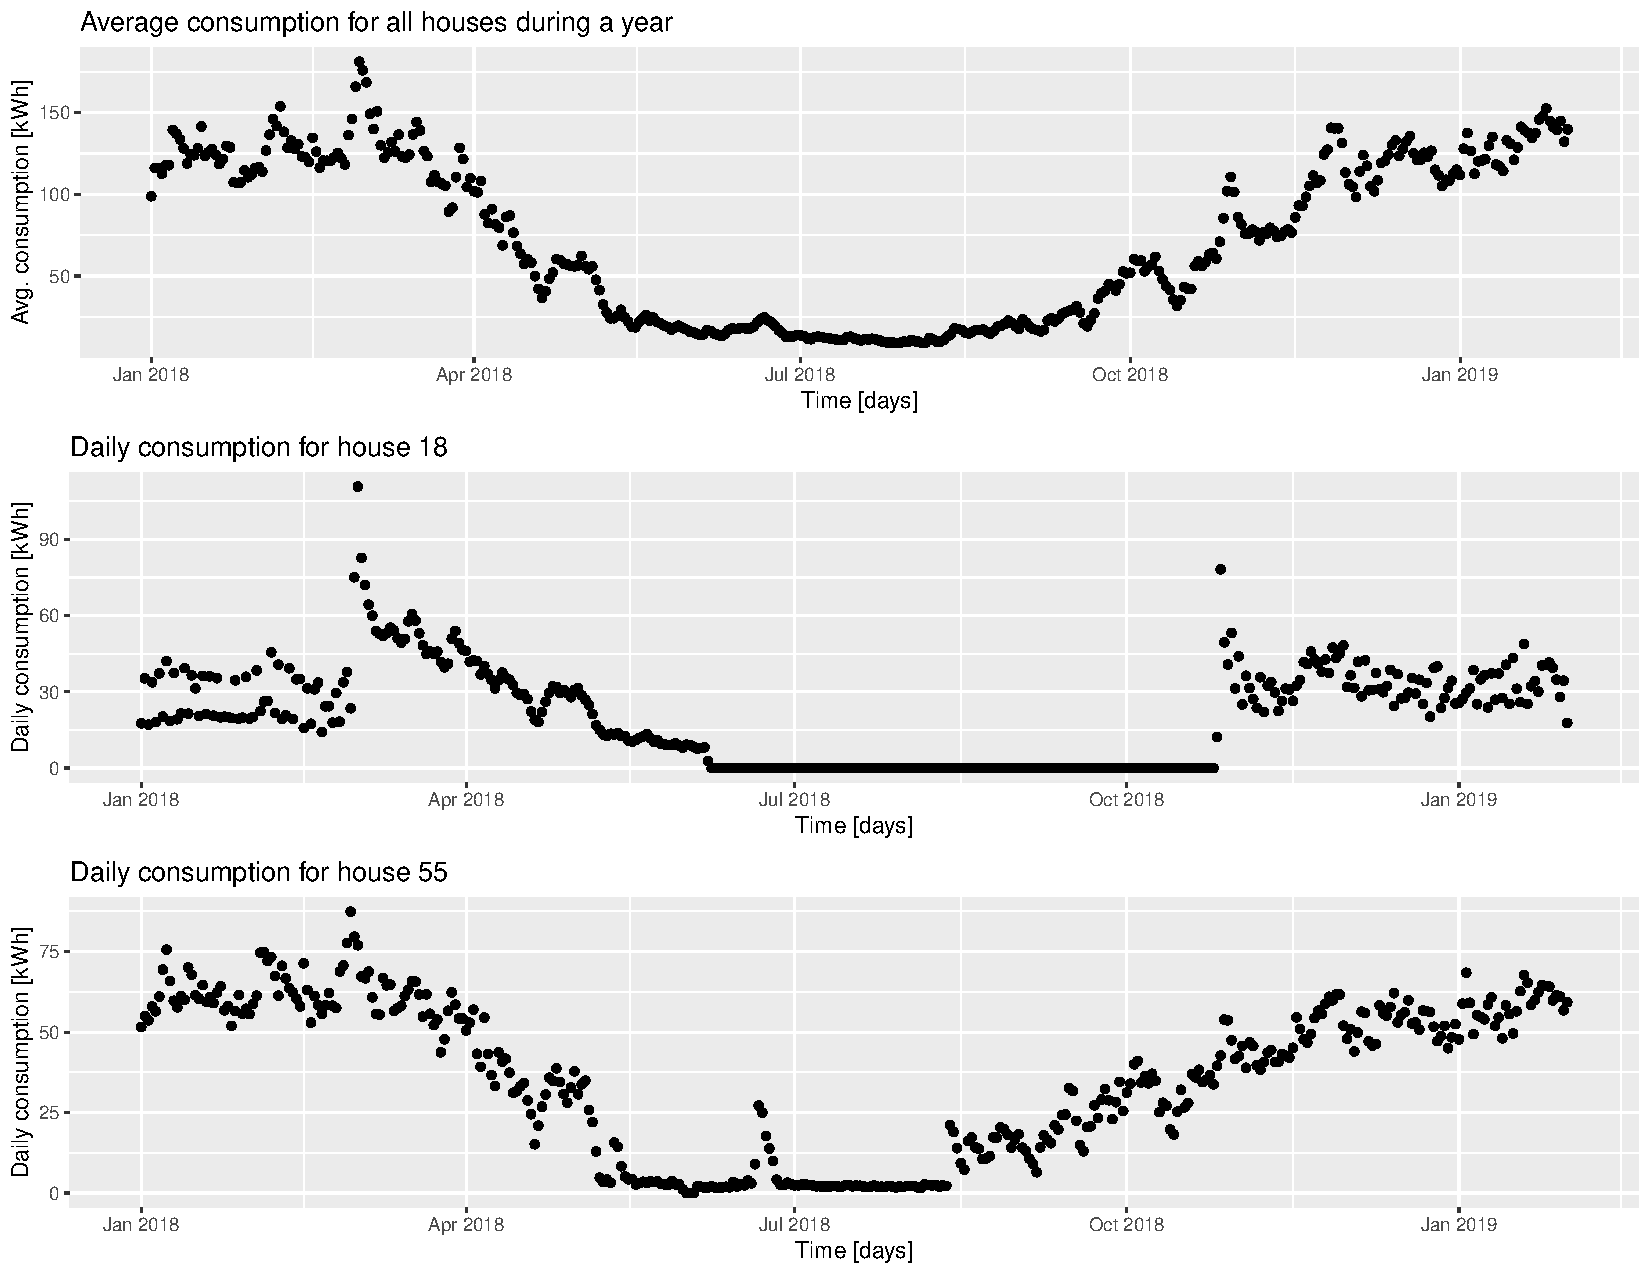
\includegraphics[width=1.\textwidth]{../../../figures/daily_cons.pdf}
    \caption{}
    \label{fig:}
\end{figure}


The figure (de udvalgte weather pairs) shows the dependencies between the average consumption of the houses and the weather attributes.
We already know that there is a dependency between the consumption and the time of year. During the summer period there
is almost no consumption. The consumption in this period is probably mostly tap water. The next important thing is the relation
between temperature and consumption. High temperatures tend to imply a higher consumption. And the reason why the consumption
depends so clearly on the time of year can be assumed to that certain periods have similar temperature levels. 
It can 

